\chapter{Infraestructura utilizada}\label{cap.infraestructura}
\hspace{1 cm} Despues de fijar los objetivos concretos de este TFG, en este cap\'itulo se va a hablar sobre las distintas tecnolog\'ias utilizadas, tanto hardware como software, y el uso que han tenido en este proyecto. 

\section{Parrot AR.Drone 2.0 }
\hspace{1 cm} \'Este ha sido el drone utilizado para hacer las pruebas en un entorno real y comprobar as\'i que el desarrollo del algoritmo era el correcto. 

\hspace{1 cm} La \textsl{bater\'ia} era de 1500mah, siendo la duraci\'on en tiempo de vuelo de unos 12 minutos. %, lo que en algunas ocasiones nos ha llevado a problemas, pues el tiempo de vuelo con esto es unos 12 minutos aproxim\'adamente. Esto conllevaba que algunas pruebas en ocasiones eran muy dif\'iciles de realizar, ya que si no salia el resultado esperado en los primeros intentos muchas veces hab\'ia que parar la prueba durante bastante rato para continuar. Si las pruebas no eran de vuelo sino que era de imagen con este tiempo era suficiente, ya que el dron no gastaba tanta energ\'ia al relizar solo la retransmisi\'on de los datos que obten\'ia la c\'amara. Un detalle curioso en este punto es el cambio de funcionamiento que se notaba una vez la bater\'ia estaba por debajo del 30/100, pues el despegue se hac\'ia con menos fuerza y de forma m\'as inestable, adem\'as las instrucciones de movimiento que se le mandaban las ejecutaba con menos fuerza y por lo tanto de forma m\'as lenta. La \'unica soluci\'on posible para remediar este problema fue trabajar a la vez con 3 bater\'ias, pero he de decir que en momentos que las pruebas eran muy continuas durante mucho tiempo, llegaba un momento que hab\'ia que parar porque el tiempo de carga no era suficientemente rapido comparado con el de las 3 descargas. 

\hspace{1 cm} El \textsl{alcance} que tiene \'este con la estaci\'on tierra es de 50 metros, suficiente para las pruebas que han sido realizadas en este proyecto. 

\hspace{1 cm} Este dron tiene una \textsl{placa base} ARM Cortex A8 de 1Ghz y un DSP de v\'ideo de 8Ghz. Tambi\'en posee una memoria RAM DDR2 de 1GB y 200Mhz. Este chip es el encargado de levantar una red WiFi, a la cual nos podemos conectar mediante el smartphone (hay una aplicacion espec\'ifica para ello), o como en este caso, mediante el ordenador, y de esta forma poder controlarlo. Esta placa base funciona con Linux. 

\hspace{1 cm} Adem\'as, dicho dron cuenta con dos \textsl{c\'amaras}, una horizontal y otra vertical, lo que nos permite ver diversos planos en todo momento. Estas c\'amaras est\'an conectadas a la placa base, lo que permite en todo momento la transmisi\'on de im\'agenes en directo, gracias a las cuales podremos trabajar, ser\'a la informaci\'on gracias a la cual podremos darle instrucciones al dron. %Cabe destacar la diferencia de calidad que hay entre las c\'amaras, algo que se notaba al realizar pruebas con una c\'amara, y cuando todo era correcto y quer\'ias cambiar de c\'amara para realizar otra prueba, se pod\'ia observar como los colores perd\'ian nitidez y se despreciaban algunos detalles, lo que te llevaba a cambiar cosas de los algoritmos que en un principio no se esperaban. 

\hspace{1 cm} Ya para terminar, la \textsl{velocidad} de este drone puede llegar a alcanzar los 18km/h, algo que en este proyecto nunca he llegado a probar, pero ser\'ia algo poco aconsejable teniendo en cuenta la distancia de alcance, pues los 50 metros que tiene, si la estaci\'on terrena de comunicaci\'on esta en un punto fijo, el dron tardar\'ia 10 segundos en salirse de este rango. 


\section{Simulador Gazebo }
\hspace{1 cm} Es un proyecto de Open Source Robotics Fundation distribuido bajo la licencia Apache 2.0. Durante este trabajo se ha trabajado con Gazebo 7. 

\hspace{1 cm}Tiene la capacidad de simulad de forma precisa ambientes con robots, objetos y sensores en distintos tipos de entonos. Por esto, nos permite trabajar con el Parrot ArDrone, y de esta forma poder probar los distintos avances que se iban realizando. \'Este nos permit\'ia realizar pruebas sin tener que preocuparnos por el material ni los daños que e podian causar. Gazebo permite la creaci\'on de entornos de manera precisa y poder probar los robots en distintos tipos de ambientes. Se trata de un programa OpenSource, lo que ha permitido su expansi\'on con facilidad, y muchos añadidos como plugins o repositorios con robots comerciales para poder acceder a su uso. Esta plataforma ha sido en la que se ha trabajado principalmente durante todo el proyecto, pues existe en \'esta un simulador de ArDrone. El escenario principal aqu\'i utilizado consist\'ia en el dron y un coche con una baliza, el cual ten\'ia que encontrar, centrarse sobre ella y aterrizar.

\hspace{1 cm} Destacar que este simulador se utiliz\'o en el DARPA Robotics Challenge, programa que trata de abordar problemas de operaciones humanitarias, como son casos de socorro en desastres naturales, que pueden ser demasiado grandes para que el ser humano se enfrente a ellos y responda de forma adecuada.

\begin{figure}[H]
	\centering
		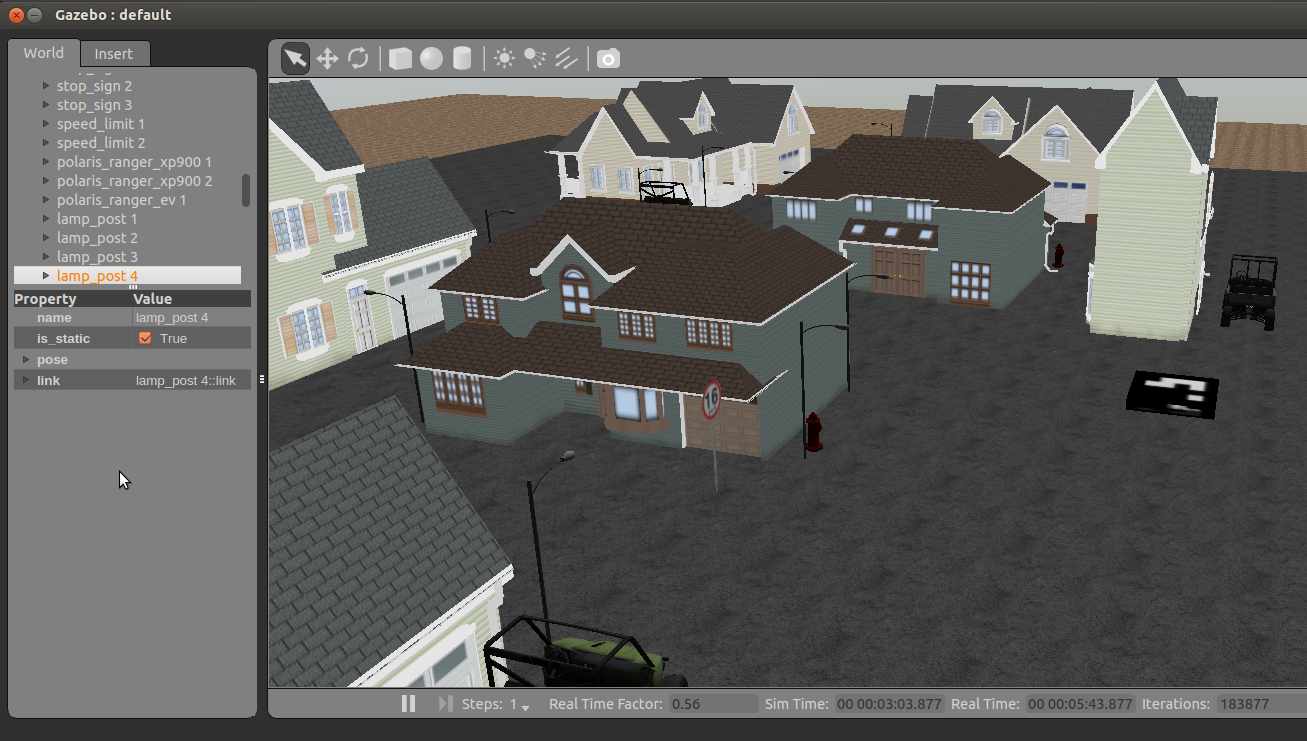
\includegraphics[width=0.5\textwidth]{imgs/gazeboworld.png}
				\caption{Mundo Gazebo.}
	\label{fig:MundoGazebo}
\end{figure}

\section{Entorno JdeRobot}
\hspace{1 cm} Este es el software principal con el que se ha trabajado, cuya web oficial es \underline{\url{www.jderobot.org}}. Se trata de un proyecto de software libre que se centra en la rob\'otica y en la visi\'on por computaci\'on. Este software cuenta con distintas herramientas como filtro de color o control de los diferentes robots, que ha permitido un continuo desarrollo desde el inicio. 


\subsection{Driver ArDroneServer}
\hspace{1 cm} Este es el servidor que nos permit\'ia comunicar nuestra aplicaci\'on con el drone. Tiene dos partes principales. Por un lado se encuentra el ArDrone SDK, el cual se comunica con el robot a\'ereo mediante WiFi. Por otro lado se encuentra el envoltorio C++, el cual se comunica con la aplicaci\'on mediante las interfaces ICE, permitiendo de esta forma la comunicaci\'on de nuestra aplicacio\'on con el cuadricoptero. 

\subsection{Plugin modelo de cuadricoptero Gazebo}
\hspace{1 cm} Plugin que permite tener un ArDrone2 de Parrot en el simulador. Este tiene distintos sensores con los que trabajar (Sonar, IMU y C\'amara), ademas de contar con los distintos controles (cargar,iniciar, actualizar,despegue, velocidad y aterrizaje). Por otro lado cuenta con la interfaz ICE para poder comunicar con los distintos elementos. 




\subsection{Herramienta UAVviewer}
\hspace{1 cm} Esta herramienta permite el control del drone y obtener los datos de sus sensores. Su interfaz ICE tiene los drivers de Camara, Pose3D, CMDVel, NAVData y ArDrone\_Extra. 

\begin{figure}[H]
 \centering
  \subfloat[UAV\_Viewer Data]{
   \label{f:UAV_Viewer1}
    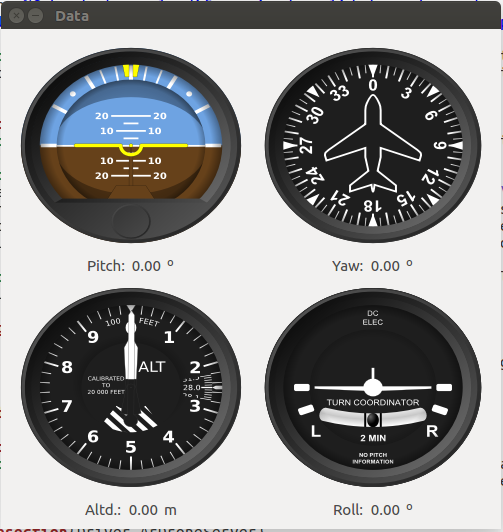
\includegraphics[width=0.29\textwidth]{imgs/UAV1.png}}
  \subfloat[UAV\_Viewer Tool]{
   \label{f:UAV_Viewer2}
    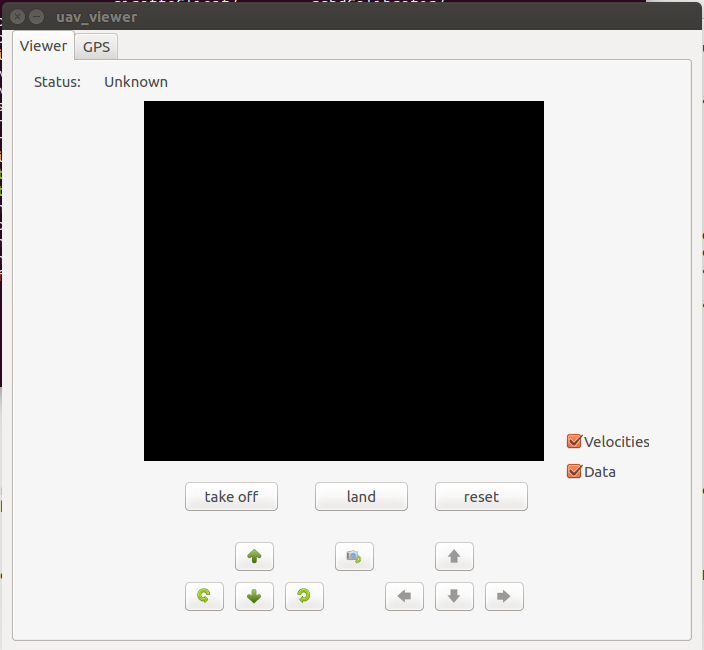
\includegraphics[width=0.33\textwidth]{imgs/UAV2.png}} 
  \subfloat[UAV\_Viewer Velocity]{
   \label{f:UAV_Viewer3}
    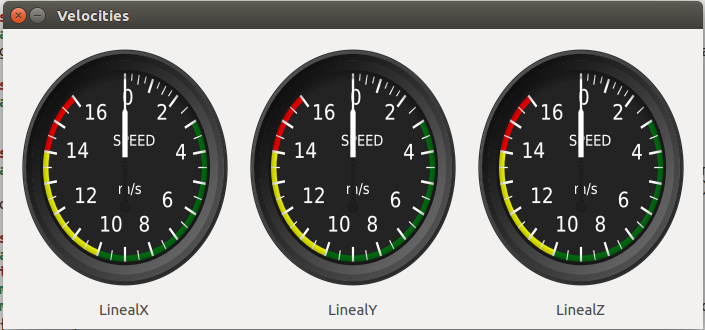
\includegraphics[width=0.25\textwidth]{imgs/UAV3.png}} 
 \caption{UAV viewer}
 \label{f:UAVViewerTotal}
\end{figure} 


\subsection{Herramienta ColorTuner}
\hspace{1 cm} Al inicio del proyecto era la herramienta ColorFilter. Esta herramienta nos permite, a partir de una imagen o v\'ideo, trabajar en los distintos espacios de color (como puede ser RGB, HSV, HSI...) y poder ir variando los parametros m\'aximo y m\'inimo (entre 0 y 255) de cada uno para ver que colores cumplen las caracter\'isticas y cuales no, viendose de esta forma, en otra imagen, s\'olo los colores que pasan este filtro dejando el resto como un fondo negro. 

\subsection{JdeRobot Academy}
\hspace{1 cm} Con esta herramienta se ha trabajado en dos secciones.
\begin{itemize}
\item 1ª Por una parte se ha utilizado para la pr\'actica de aut\'omatas. Esta nos permitia crear un diagrama de estados para saber en cada momento en que punto del algoritmo nos encontramos.

\begin{figure}[ht]
	\centering
		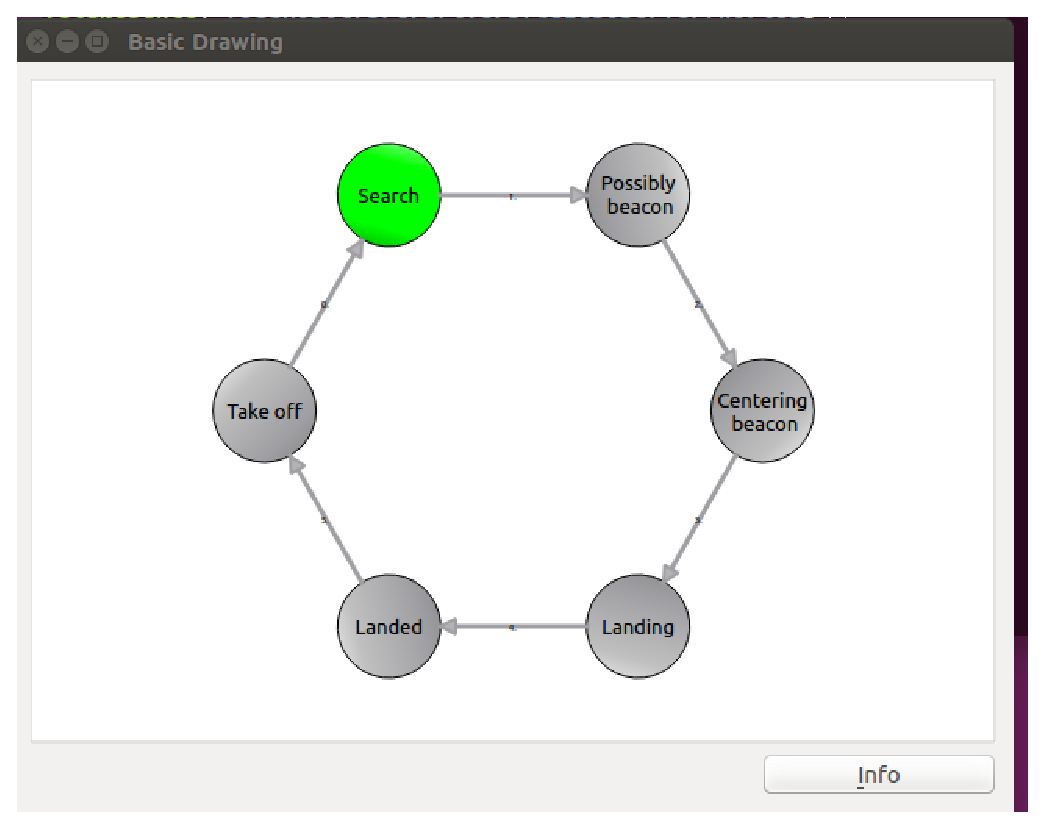
\includegraphics[width=0.3\textwidth]{imgs/states.eps}
		\caption{Diagrama de estados.}
	\label{fig:Diag_estados}
\end{figure}

\item 2ª Por otro lado se ha utilizado follow\_turtlebot, al igual que UAVviewer, nos permite controlar el drone y obtener los datos de sus sensores, adem\'as de poder ejecutar nuestro algoritmo.
 \begin{figure}[H]
	\centering
		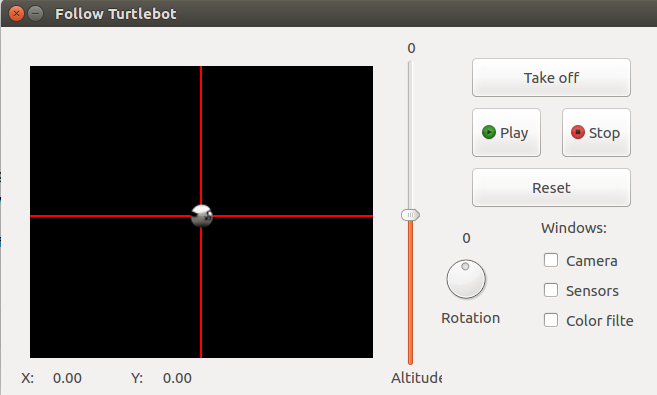
\includegraphics[width=0.5\textwidth]{imgs/follow_turtlebot.png}
		\caption{Follow Turtlebot.}
	\label{fig:FollowTurtlebot}
\end{figure}


\end{itemize}

%En primer lugar se utilizo \textit{color filter} para ver el funcionamiento de los filtros de color. Esta herramienta nos permite, a partir de una imagen o v\'ideo, trabajar en los distintos espacios de color (como puede ser RGB, HSV, HSI...) y poder ir variando los parametros m\'aximo y m\'inimo (entre 0 y 255) de cada uno para ver que colores cumplen las caracter\'isticas y cuales no, viendose de esta forma, en otra imagen, s\'olo los colores que pasan este filtro dejando el resto como un fondo negro. 
%Una vez utilizada esta herramienta y realizamos pequeños algoritmos para ver que funcionaba igual un filtro propio que este filtro, pasamos a trabajar con otra llamada \textit{follow turtleboot}. \'Esta  nos permit\'ia manejar el dron, teniendo un cuadro que nos permite el movimiento en los ejes X e Y, una barra para realizar un cambio en la altura y un pequeño c\'irculo para que pudiera rotar sobre s\'i mismo. Por otro lado ten\'ia un bot\'on para aterrizaje y despegue y unos botones que permiten iniciar un algoritmo creado, de forma que podemos probar si lo programado funciona. Esta herramienta puede sacar tres cuadros diferentes, uno para la c\'amara, el cual nos da una imagen en directo de lo que est\'a transmitiendo el dron y nos da la opci\'on de elegir la c\'amara que queremos ver. El segundo, nos muestra las distintas propiedades del dron en ese momento como la orientaci\'on, altura o inclinaci\'on. Por \'ultimo, el \'ultimo cuadro es para el filtro de color. \'Este funciona cuando el algoritmo programado est\'a en marcha. En un primer momento como indica su nombre, nos permite trabajar con el filtro de color que hab\'iamos practicado antes sobre la otra herramienta, pero al final utilizamos \'este para realizar marcas sobre la imagen de las cosas que nos interesaban de esta, como puede ser encuadrar la baliza, la cruceta o pintar sobre \'esta. 
%Por \'ultimo, a todo esto le hemos añadido un diagrama de estados, gracias a una pequeña aplicaci\'on desarrollara a partir de \textit{visualHFSM}. nos permit\'ia crear un dibujo de los diferentes estados por los que deber\'ia pasar el dron, seg\'un lo que estuviera viendo en cada momento o la acci\'on concreta que estaba realizando. De esta forma se marca en el diagrama en el estado en el que se encuentra, pudiendo saber as\'i cual ser\'ia el siguiente estado esperado y viendo que funciona de forma correcta.


\section{Biblioteca OpenCV}
\label{sec:BibliotecaOpenCV} 
\hspace{1 cm} Esta librer\'ia tiene un conjunto de funciones que sirven para el procesamiento de im\'agenes y visi\'on computerizada, cuya web oficial es \underline{\url{https://opencv.org/}}. Esta programada en C++ y es un estandar de facto en la visi\'on artifical. Para el procesamiento de im\'agenes nos hemos apoyado principalmente sobre esta, trabajando en la versi\'on 3.1. Gracias a \'esta, al obtener la imagen que nos transmit\'ia el drone pod\'iamos tanto detectar objetos como aplicar cambios sobre ella, para marcar las zonas de interes o diferentes objetos. Esta librer\'ia sirve para el procesamiento de im\'agenes y visi\'on computerizada. Nos ha permitido la realizaci\'on de filtros de color, para eliminar objetos no deseados dependiendo el momento. Adem\'as permite el uso de operadores morfol\'ogicos (erosi\'on y dilataci\'on) gracias a los cuales se evitaban imperfecciones en las im\'agenes como pod\'ia ser el ruido, que clasificaba objetos inexistentes o de no inter\'es como objetos de inter\'es, as\'i como zonas importantes las detectaba como p\'ixeles de fondo. Tambi\'en han sido de gran utilidad funciones como \textit{drawContours} \'o \textit{findContours}, las cuales permit\'ian encontrar los bordes de los objetos e indicar sobre una imagen final, con otro color, donde se encontraban dichos objetos. 



\begin{figure}[H]
 \centering
  \subfloat[Logo OpenCV]{
   \label{f:LogoOpenCV}
    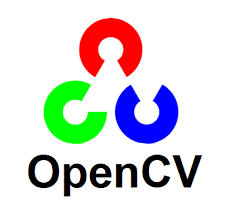
\includegraphics[width=0.29\textwidth]{imgs/opencv.png}}
  \subfloat[Procesamiento con OpenCV]{
   \label{f:OpenCVProcess}
    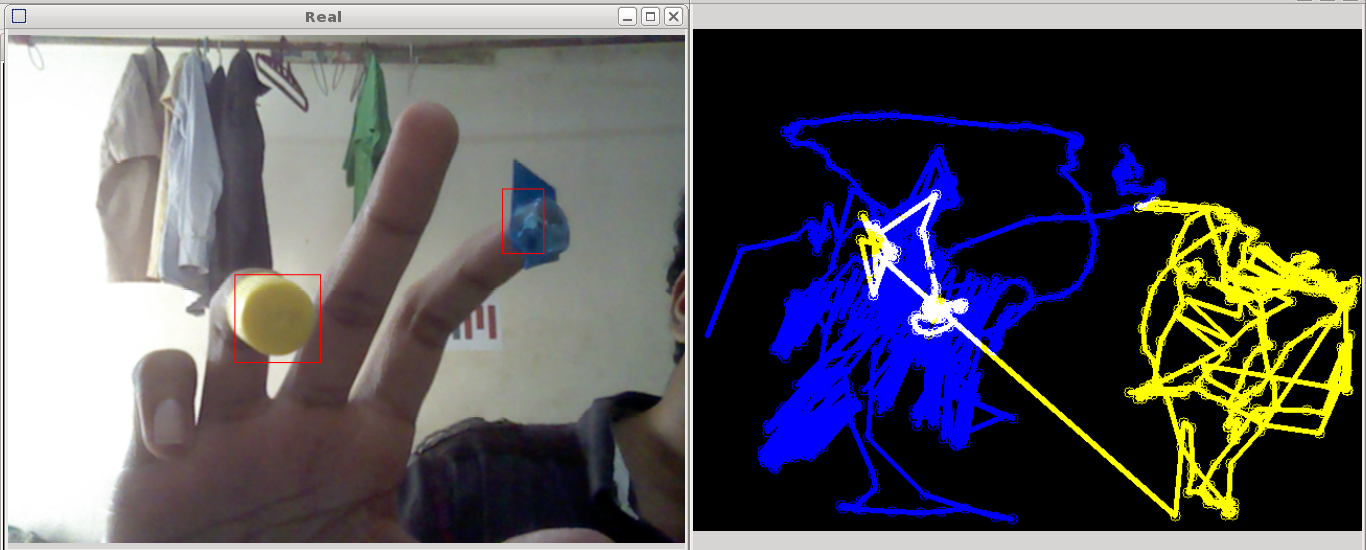
\includegraphics[width=0.33\textwidth]{imgs/opencvP.png}} 
 \caption{UAV viewer}
 \label{f:OpenCV}
\end{figure} 









